




\documentclass{beamer}[12pt]




\usepackage[utf8]{inputenc}
\usepackage{pgf}
\usepackage{amsmath,amssymb}
\usepackage{colortbl}
\usepackage{graphicx}
\usepackage{url}
\usepackage{pstricks}
\usepackage{xspace}
\usepackage{multirow}
\usepackage{eurosym}
\usepackage{beamerthemeshadow}
\beamersetuncovermixins{\opaqueness<1>{25}}{\opaqueness<2->{15}}

\usepackage[T1]{fontenc}  
\usepackage[francais]{babel}

\newcommand{\quota}[1]{\glqq{}#1\grqq{}}
\definecolor{lightred}{rgb}{1,0.3,0.3}
\definecolor{lightgreen}{rgb}{0.3,1,0.3}
\definecolor{lightblue}{rgb}{0.5,0.5,1}
\definecolor{darkred}{rgb}{0.7,0,0}
%\newcommand{\redmathbox}[1]{\colorbox{lightred}{\ensuremath{#1}}}
%\newcommand{\greenmathbox}[1]{\colorbox{lightgreen}{\ensuremath{#1}}}
%\newcommand{\pseudomathbox}[1]{\setlength{\fboxrule}{0pt}\fbox{\ensuremath{#1}}\setlength{\fboxrule}{1pt}}

\newcommand{\redbox}[1]{\colorbox{lightred}{#1}}
\newcommand{\greenbox}[1]{\colorbox{lightgreen}{#1}}
\newcommand{\bluebox}[1]{\colorbox{lightblue}{#1}}
\newcommand{\yellowbox}[1]{\colorbox{yellow}{#1}}

\setlength{\fboxrule}{1pt}


%% Das Layout
\setbeamertemplate{footline} %% Eine Fußzeile für die Slide-Nummern
{%
  \hbox{%
  \begin{beamercolorbox}[wd=.25\paperwidth,ht=2.25ex,dp=1ex,center]{author in head/foot}%
    \usebeamerfont{title in head/foot}\insertshortauthor
  \end{beamercolorbox}%
  \begin{beamercolorbox}[wd=.5\paperwidth,ht=2.25ex,dp=1ex,center]{title in head/foot}%
    \usebeamerfont{title in head/foot}\insertshorttitle
  \end{beamercolorbox}%
  \begin{beamercolorbox}[wd=.25\paperwidth,ht=2.25ex,dp=1ex,center]{date inhead/foot}%
    \insertframenumber{} / \inserttotalframenumber
    \hspace*{2ex}
  \end{beamercolorbox}}%
  \vskip0pt%
}
%\usefonttheme[onlysmall]{structurebold} %% Schriftlayout
\setbeamercovered{transparent}
%\setbeamertemplate{navigation symbols}{} %% Abschalten der Navigation

 \AtBeginSection[]
 {
   %\logo{}
   \begin{frame}
     %\frametitle{Übersicht}
     \tableofcontents[current,hideothersubsections,subsectionstyle=show/shaded/hide,subsubsectionstyle=show/shaded/hide]
   \end{frame}%\note{}
 }

\title{Gene prediction with hidden Markov models}
\subtitle{INF 582 - Datamining}
\author[T. Rohrmann \& D. Arnol]{Till Rohrmann \& Damien Arnol}
\institute{École Polytechnique}
\date{\today}

% ----------------------------------------------- BEGINNING OF THE DOCUMENT ----------------------------------------------- %
%% Das Dokument
\begin{document}

\frame{
	\titlepage
}



\begin{frame}
\frametitle{Motivation}
	\begin{figure}[h]
		\centering
		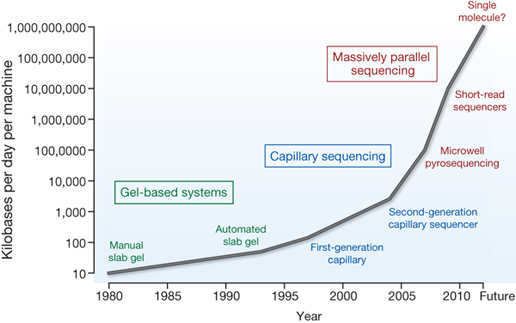
\includegraphics[width=1.0\textwidth]{../picturesforthepresentation/wtdv027274.jpg}<1>
		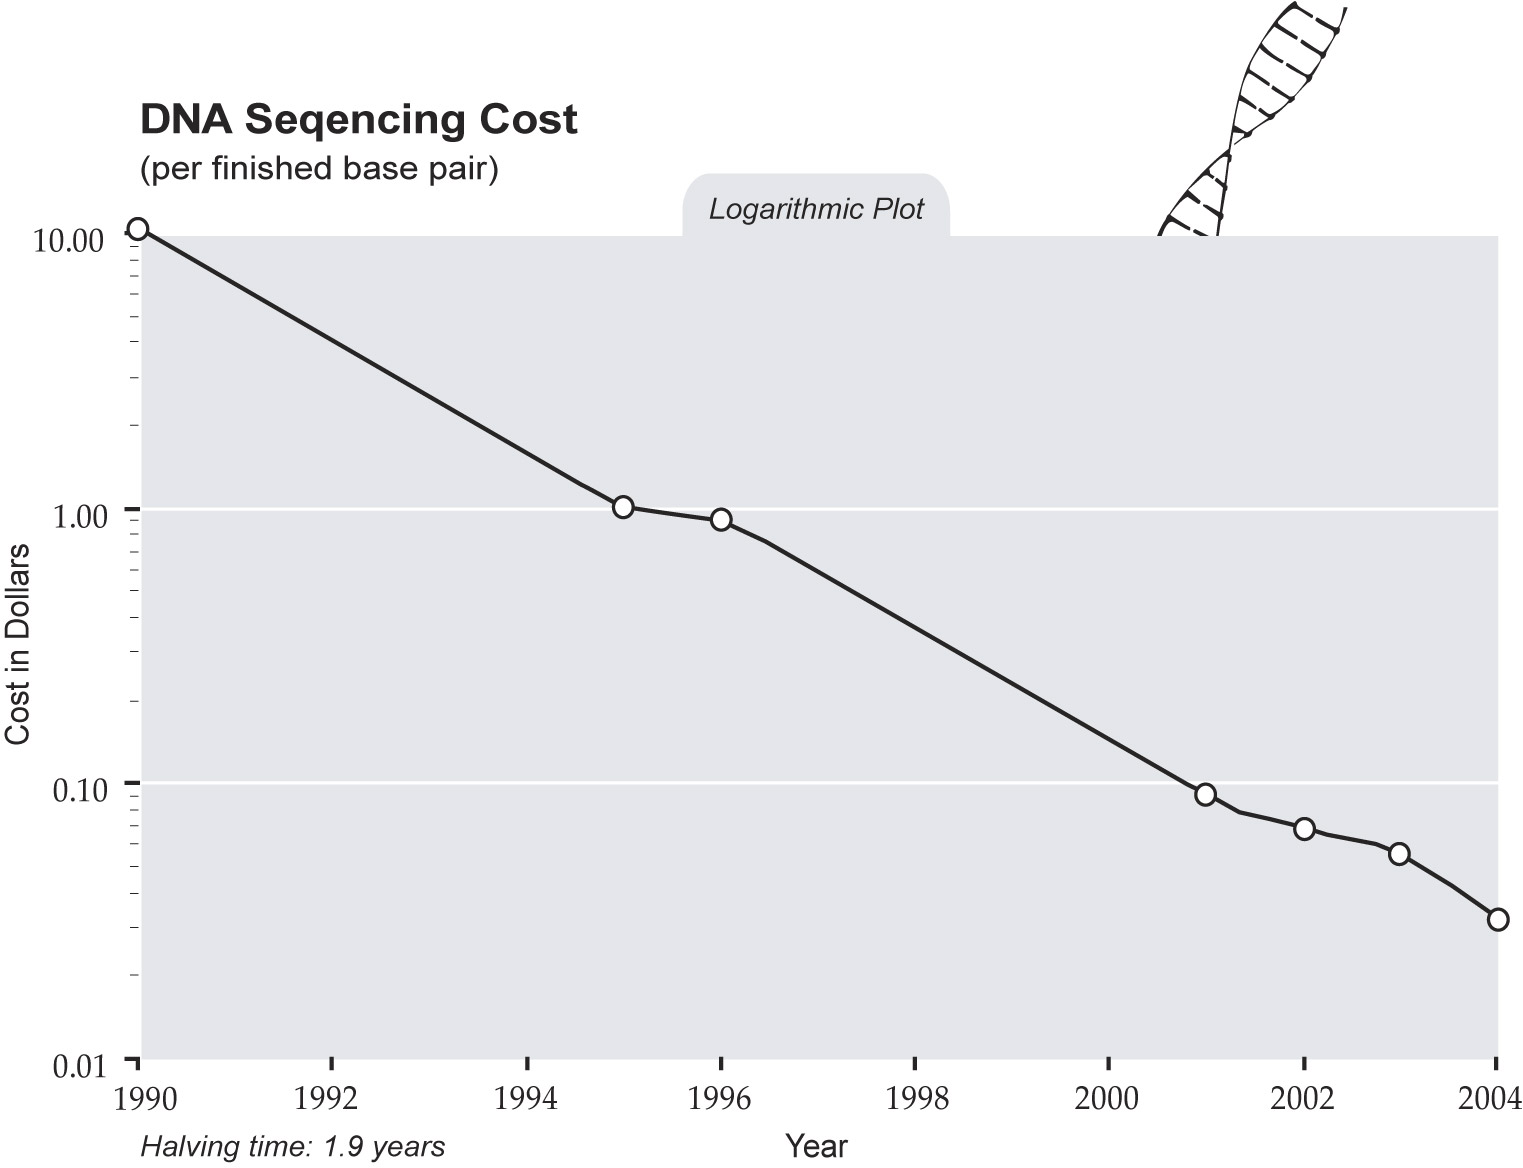
\includegraphics[width=0.85\textwidth]{../picturesforthepresentation/DNAsequencingCost.jpg}<2>		
	\end{figure}
\end{frame}


\frame{
  \frametitle{Outline}
  \tableofcontents[hideallsubsections]
}


\section{HMMs}
\subsection{Description of the probabilistic model}

\begin{frame}
\frametitle{Description of the probabilistic model}
\begin{columns}

		\column{0.50\textwidth}
		\begin{figure}[h]
			\centering
			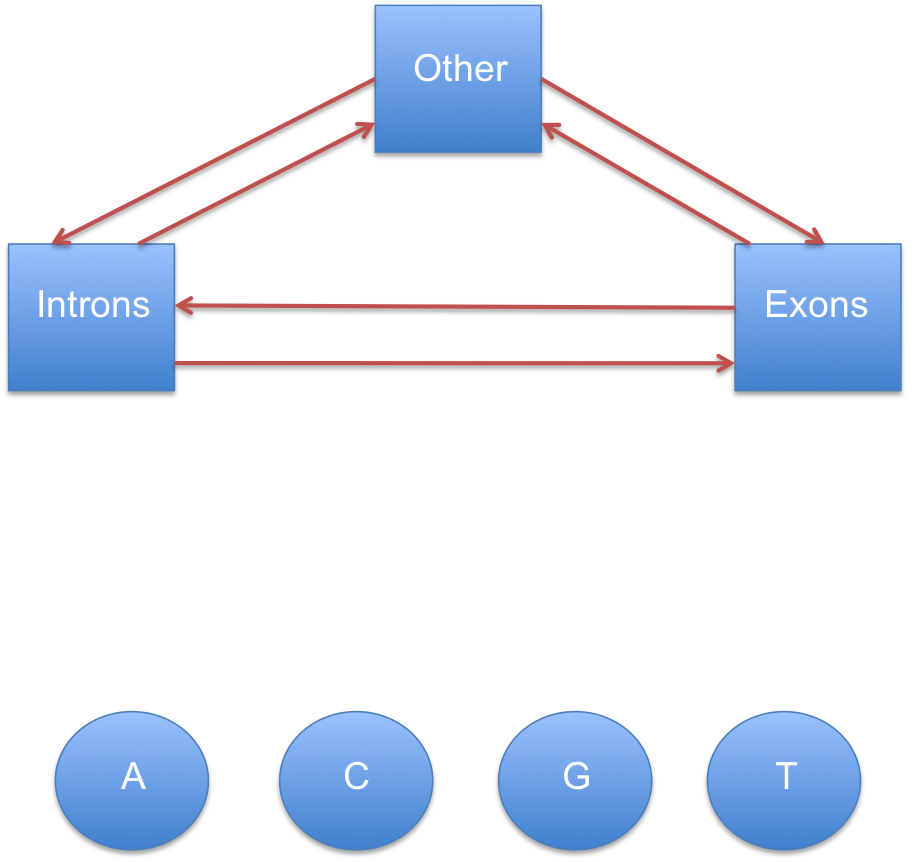
\includegraphics[width=1.0\textwidth]{../picturesforthepresentation/HMM1.png}<1>
			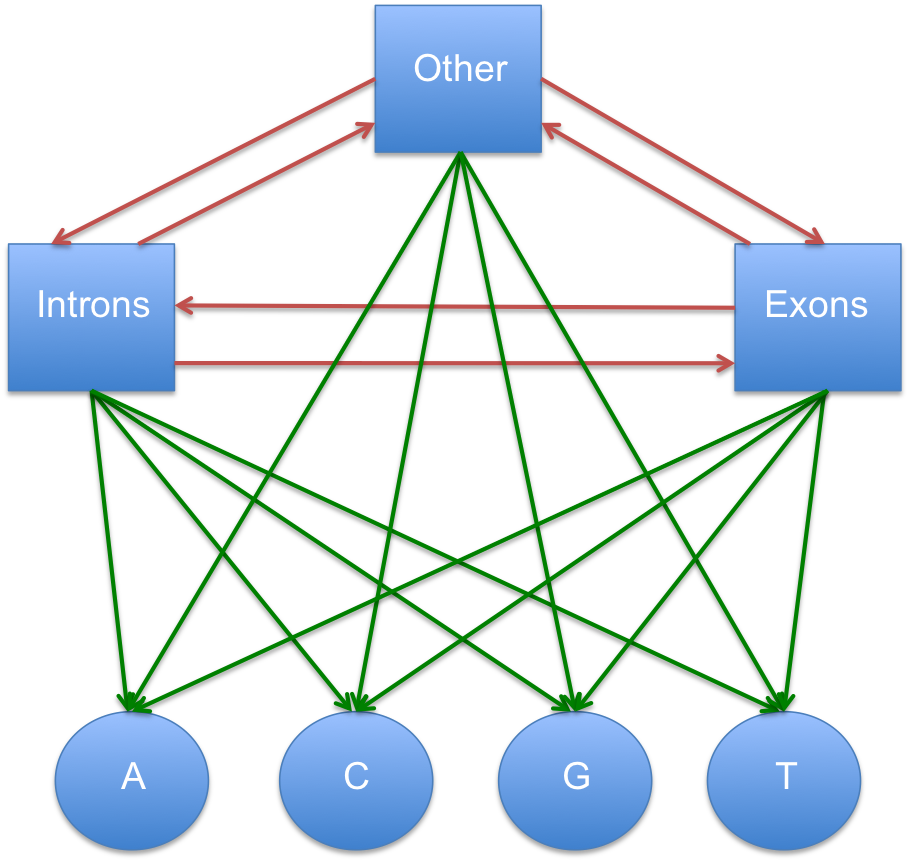
\includegraphics[width=1.0\textwidth]{../picturesforthepresentation/HMM2.png}<2>		
		\end{figure}
		
		\column{0.50\textwidth}
		\begin{block}{Transition probabilities}<1->
		%\vspace{0.1cm}
			Transition from state i to state j: $T_{ij}$\\
		
		\end{block}
		\vspace{0.3cm}
		\begin{block}{Emission probabilities}<2>
		%\vspace{0.1cm}
			Emission of A being in state i: $E(A|i)$
		\end{block}
\end{columns}
\end{frame}

\subsection{Decoding a sequence of emitted states}

\begin{frame}
\frametitle{The Viterbi algorithm}

		\begin{figure}[h]
			\centering
			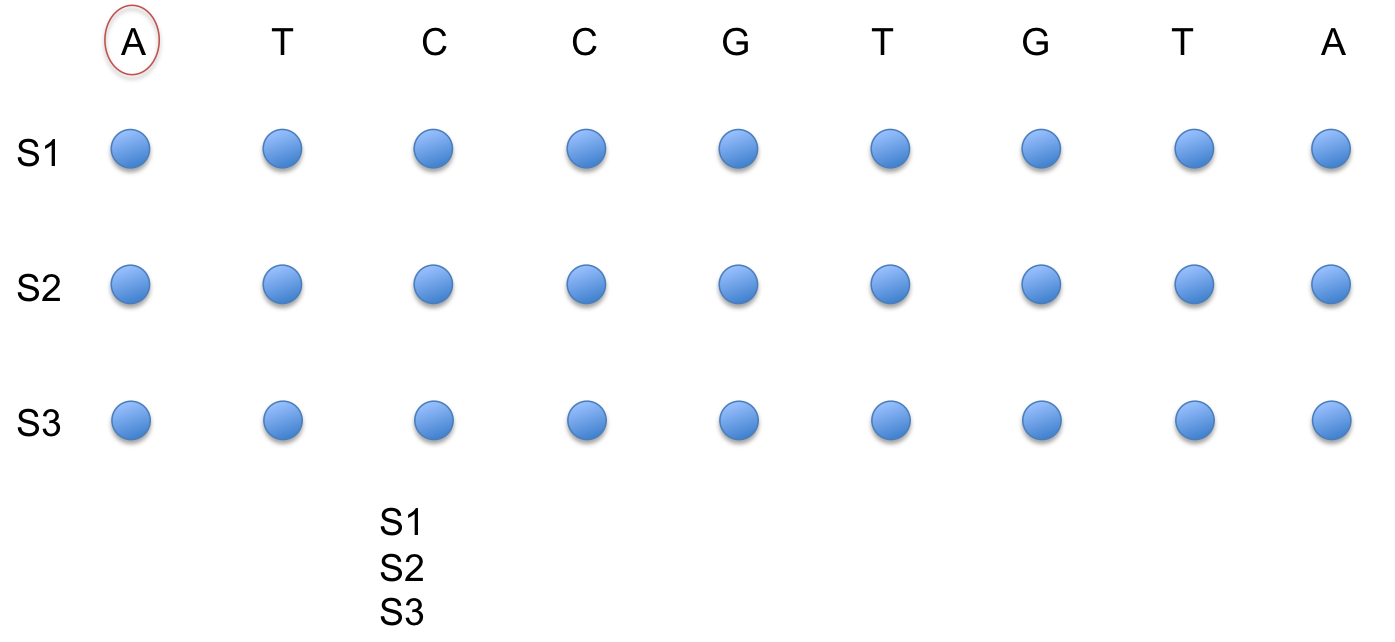
\includegraphics[width=1.0\textwidth]{../picturesforthepresentation/Viterbi1.png}<1>
			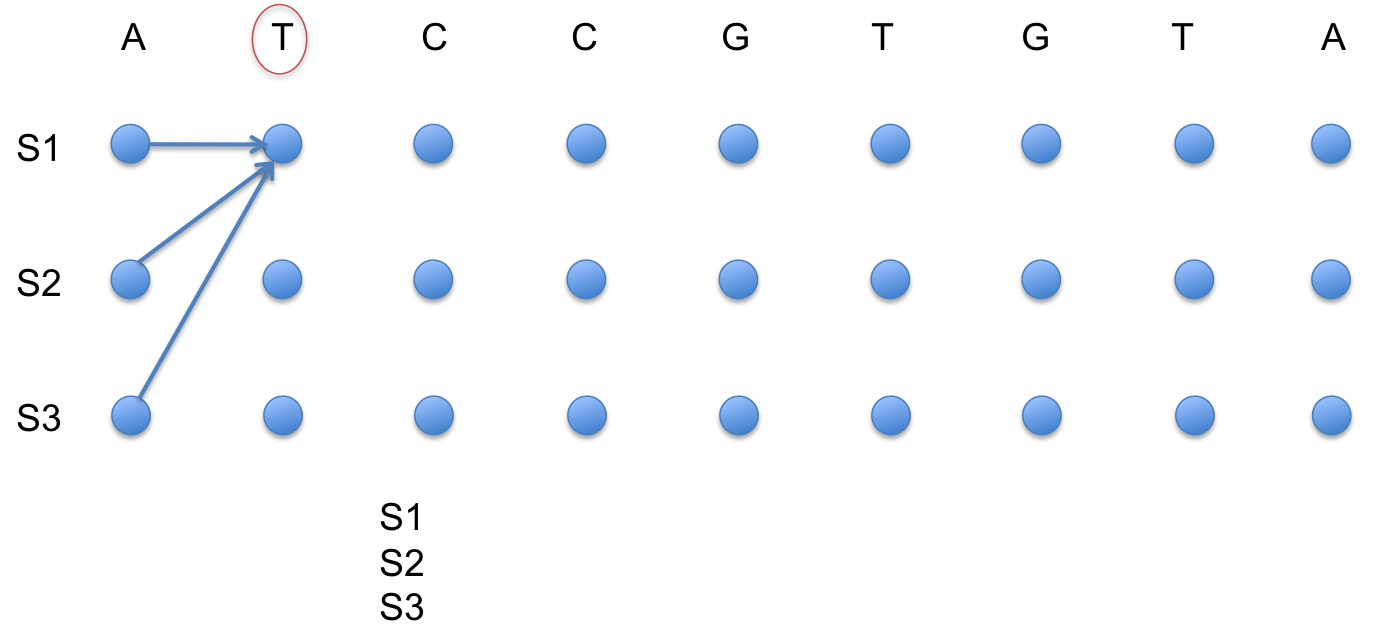
\includegraphics[width=1.0\textwidth]{../picturesforthepresentation/Viterbi2.png}<2>
			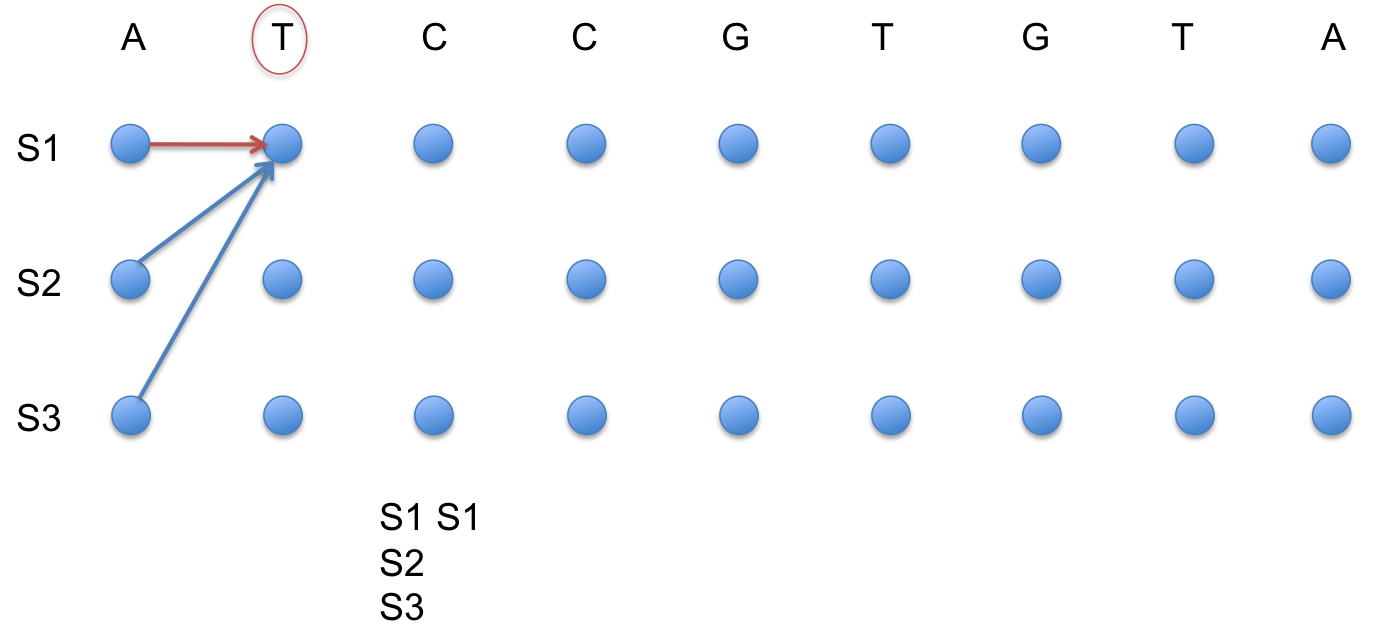
\includegraphics[width=1.0\textwidth]{../picturesforthepresentation/Viterbi3.png}<3>
			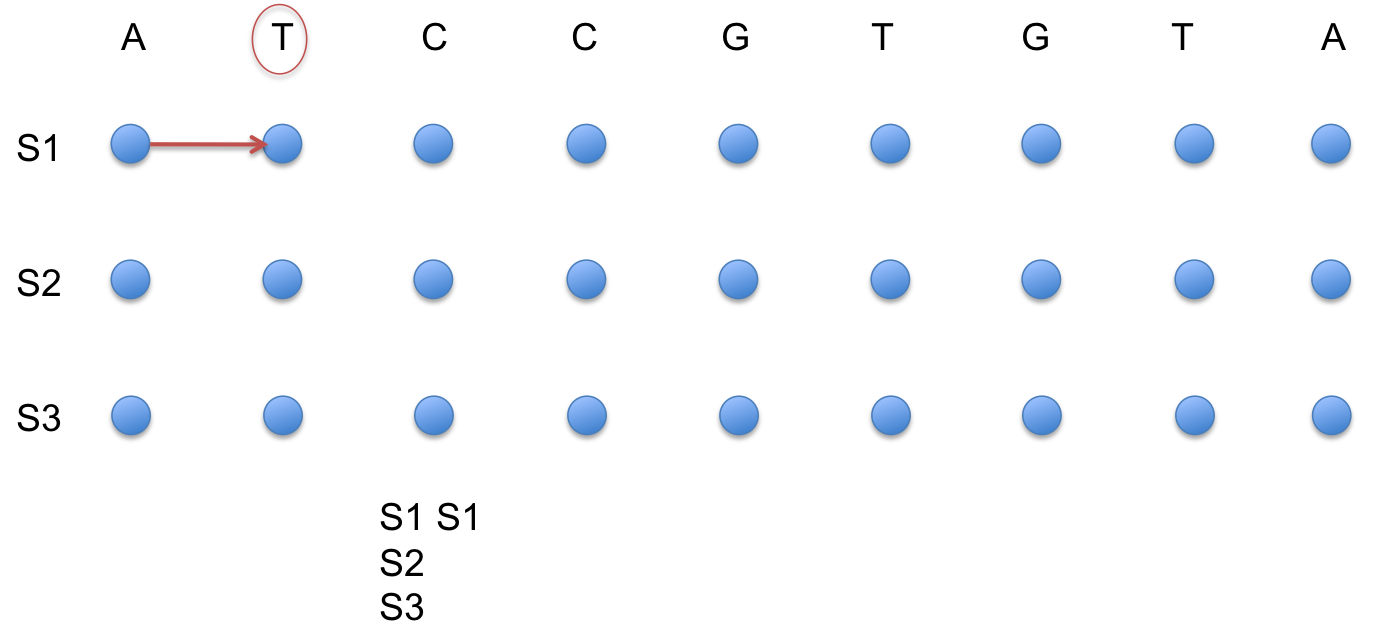
\includegraphics[width=1.0\textwidth]{../picturesforthepresentation/Viterbi4.png}<4>
			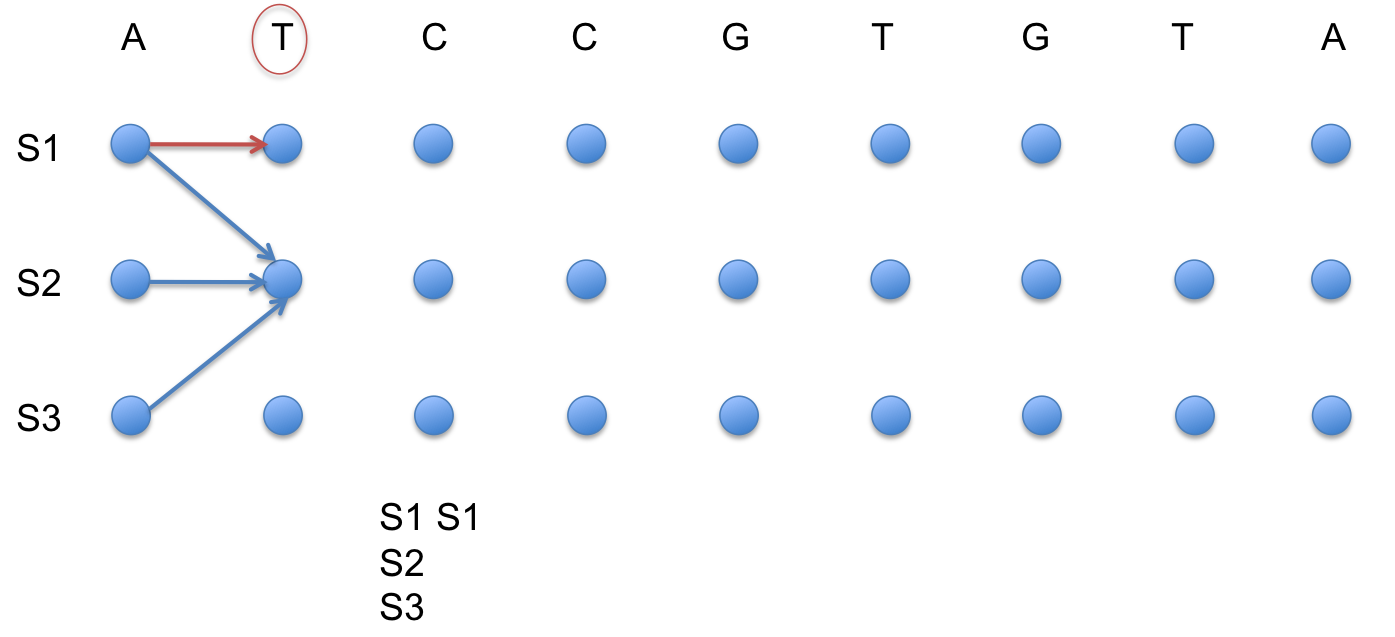
\includegraphics[width=1.0\textwidth]{../picturesforthepresentation/Viterbi5.png}<5>
			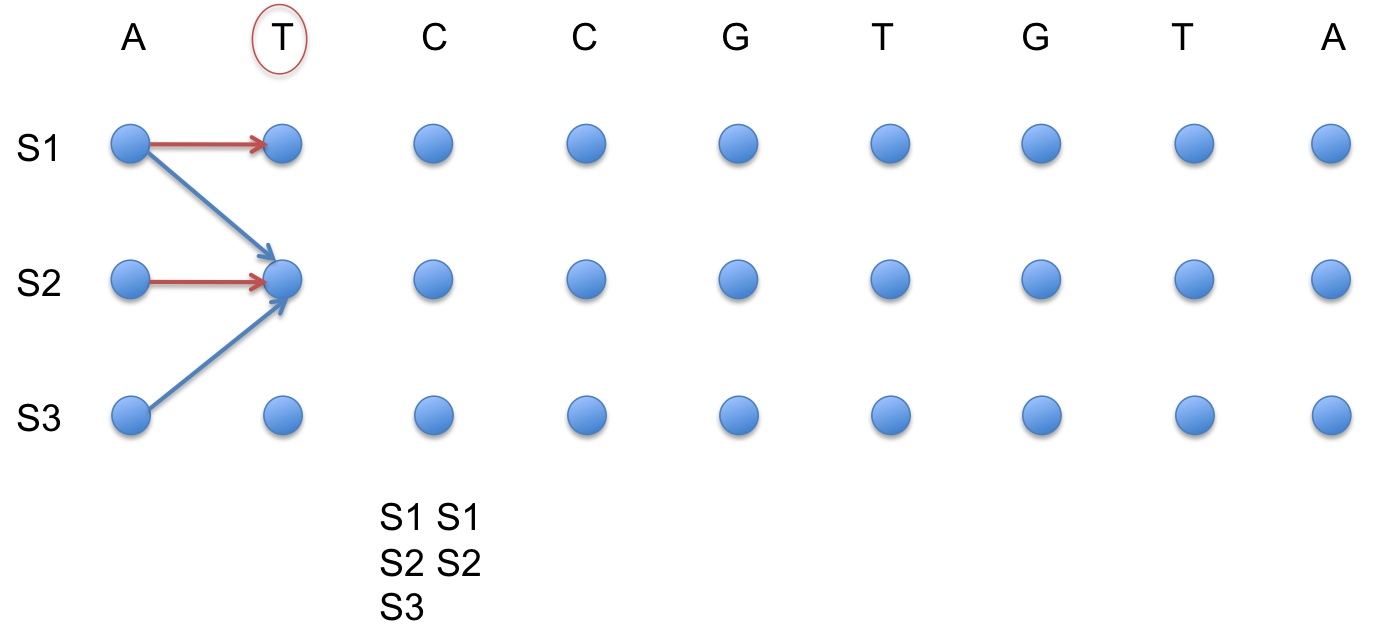
\includegraphics[width=1.0\textwidth]{../picturesforthepresentation/Viterbi6.png}<6>
			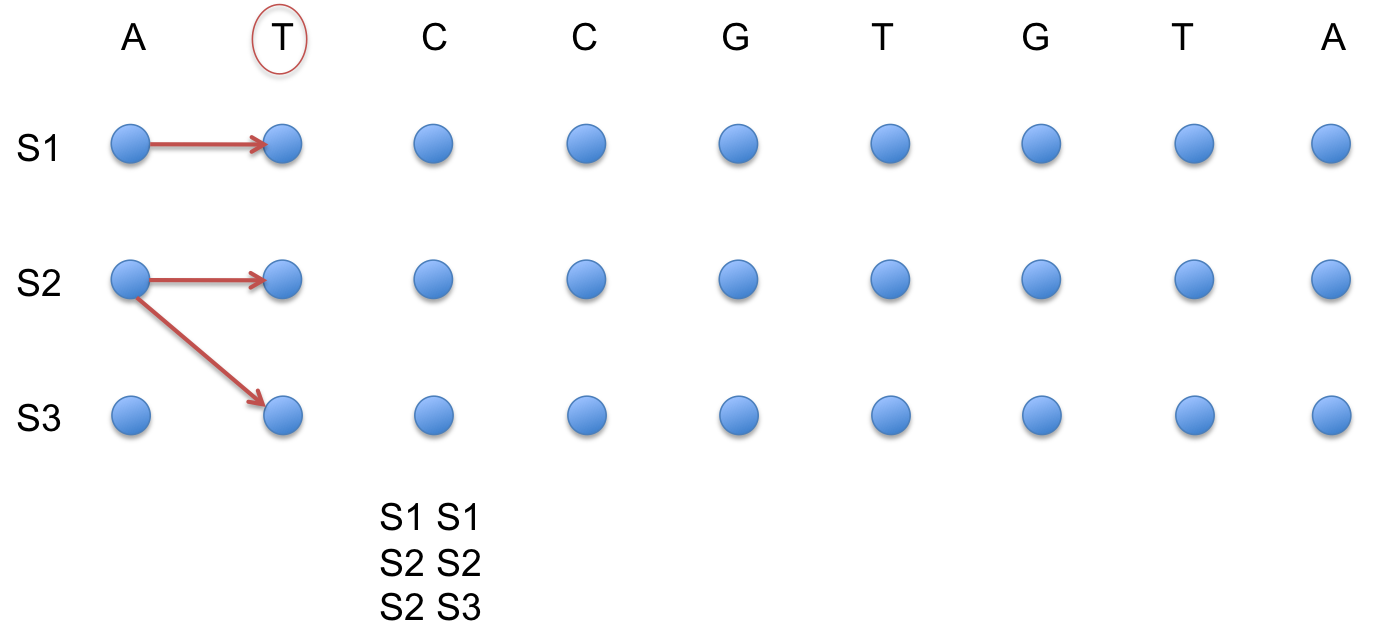
\includegraphics[width=1.0\textwidth]{../picturesforthepresentation/Viterbi7.png}<7>
			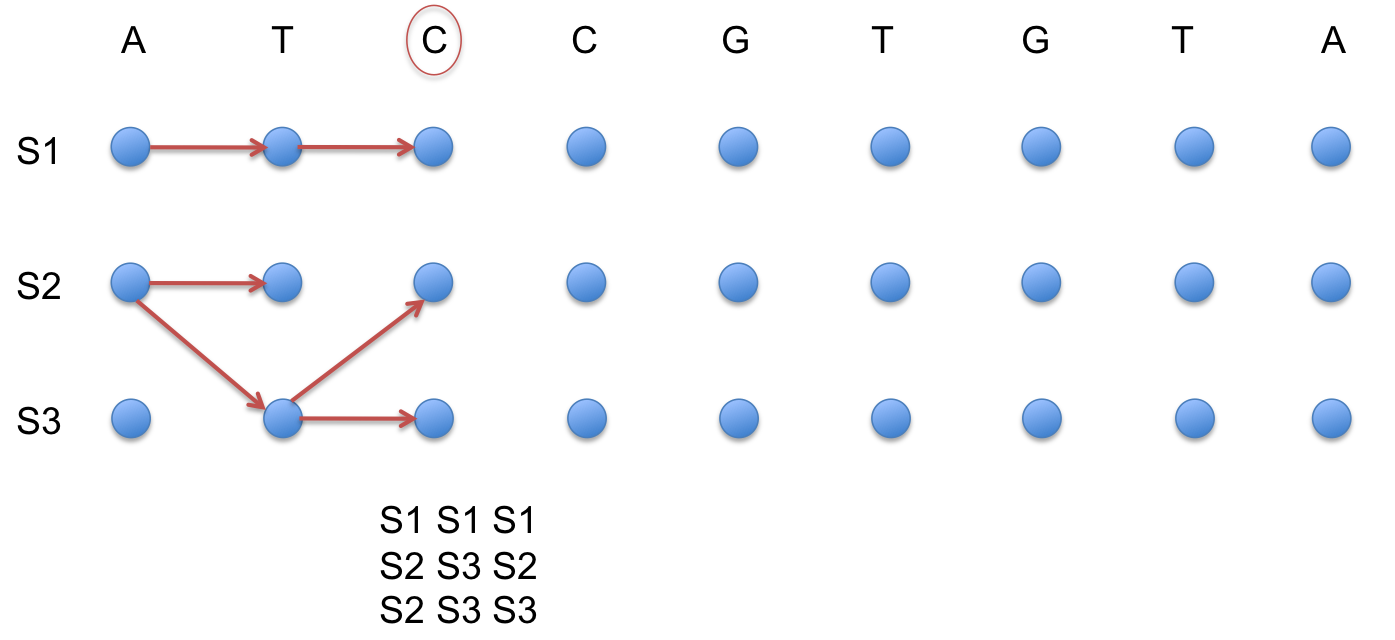
\includegraphics[width=1.0\textwidth]{../picturesforthepresentation/Viterbi8.png}<8>
			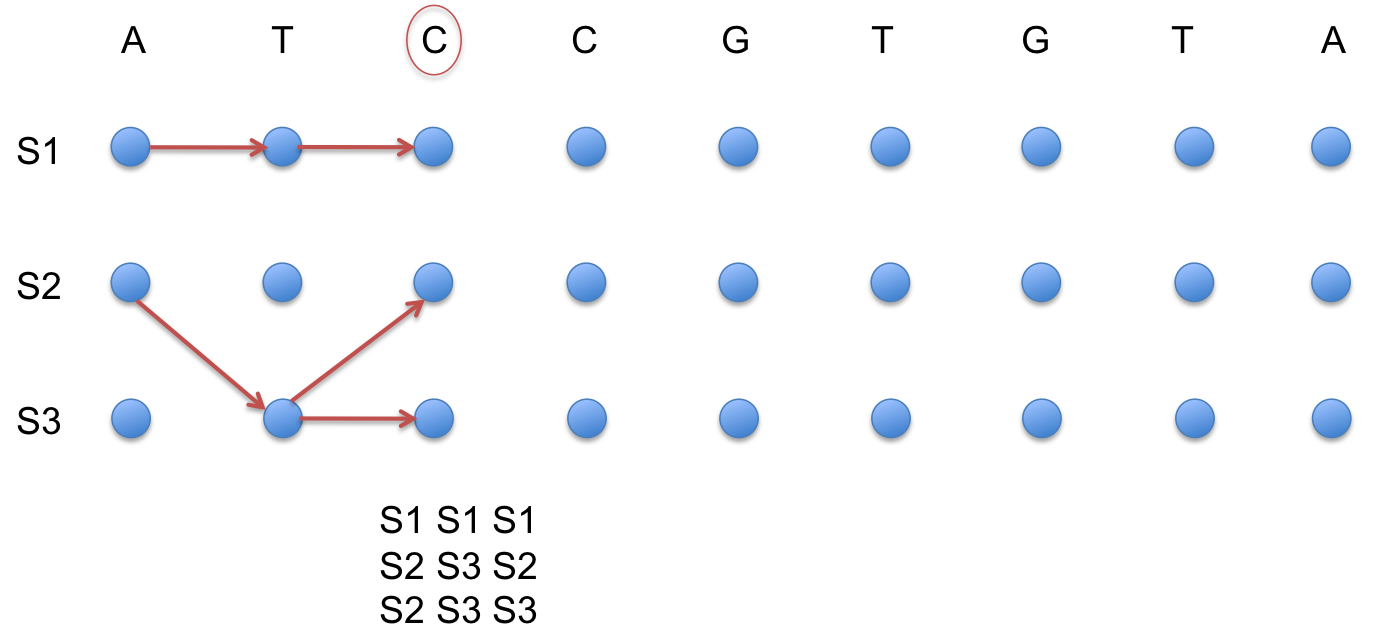
\includegraphics[width=1.0\textwidth]{../picturesforthepresentation/Viterbi9.png}<9>
			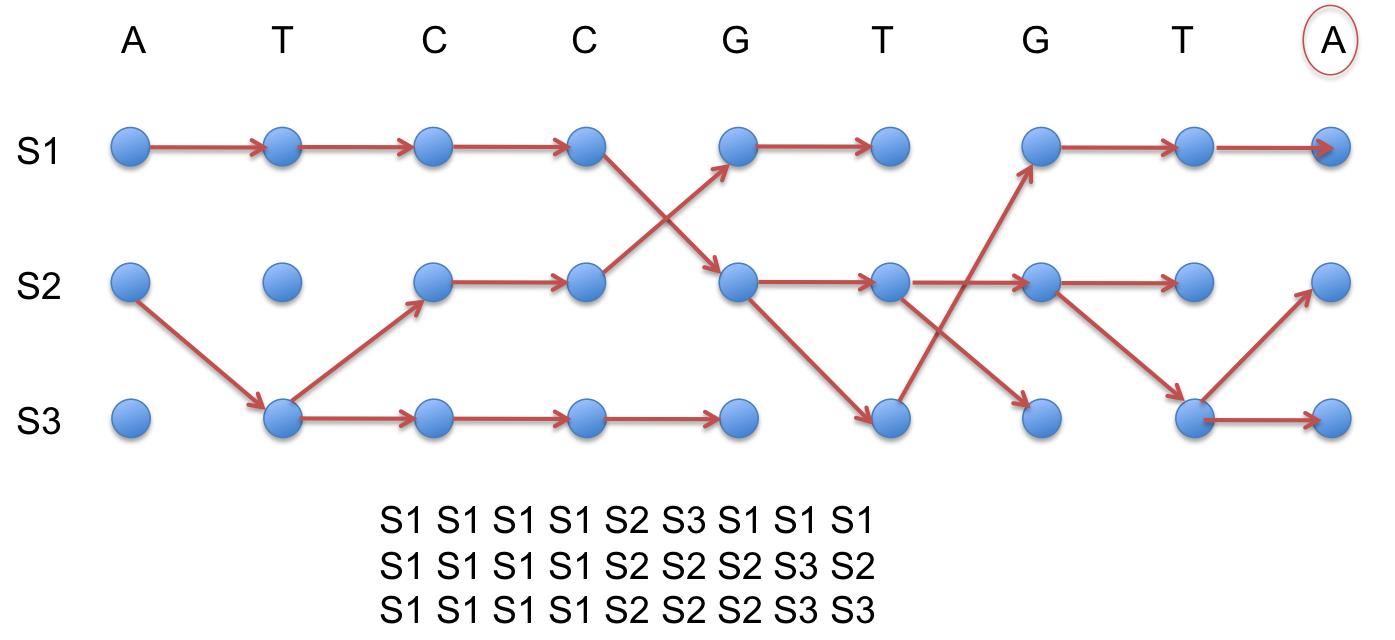
\includegraphics[width=1.0\textwidth]{../picturesforthepresentation/Viterbi10.png}<10>
			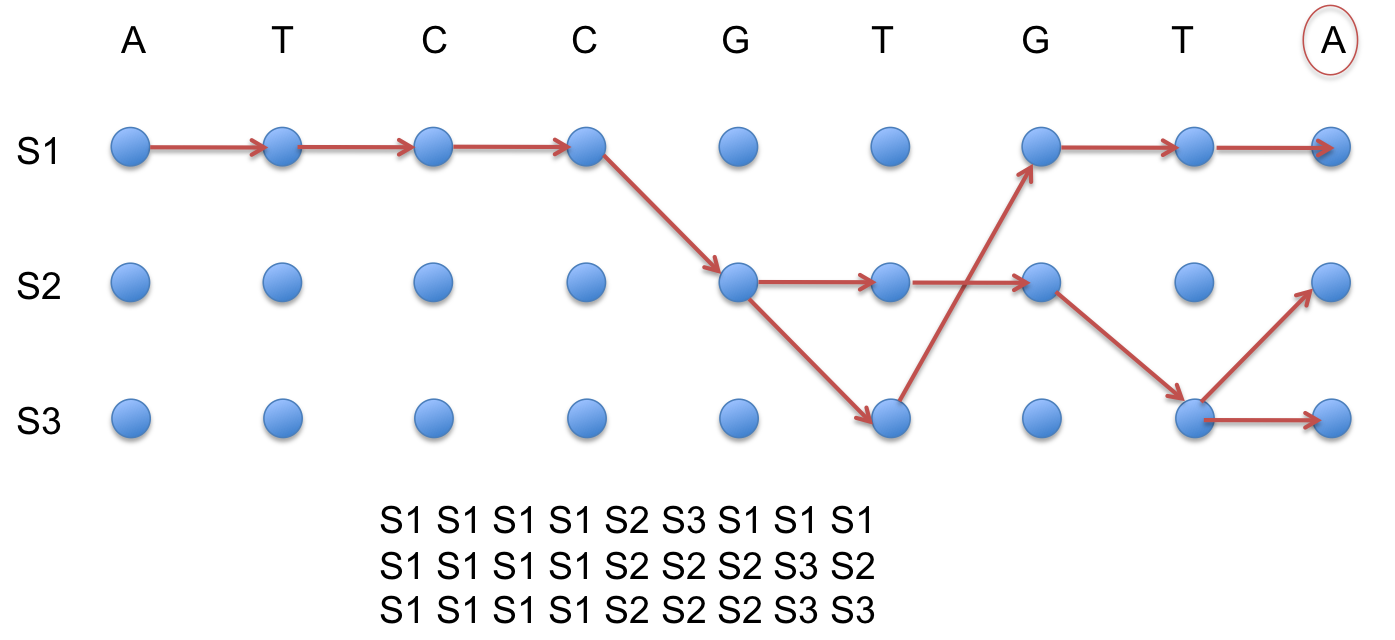
\includegraphics[width=1.0\textwidth]{../picturesforthepresentation/Viterbi11.png}<11>
			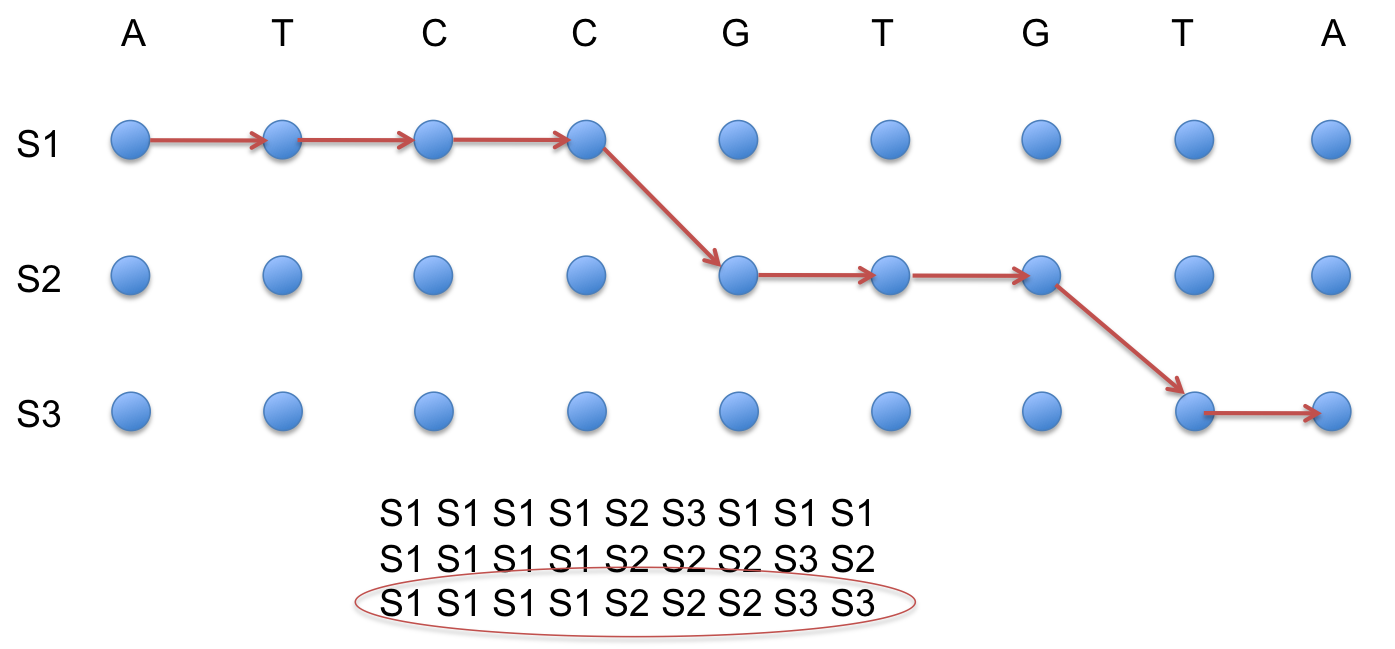
\includegraphics[width=1.0\textwidth]{../picturesforthepresentation/Viterbi12.png}<12>			
		\end{figure}

\end{frame}


\begin{frame}
\frametitle{Formal writing}

\begin{block}{Additional notations}
	\begin{tabular}{l@{\hspace{0.1em}}c@{\hspace{0.5em}}l@{\hspace{0.5em}}}
		$(y_1...y_n)$ &:& Sequence of bases to decode\\
		$S$ &:& Space of the possible states\\
		$\pi_{k}$ &:& Probability of beginning in state k\\
		$V_{t,k}$ &:& Probability of the best track ending in state k at step t
	\end{tabular}
\end{block}

\begin{block}{Initialization}
\begin{equation*}
V_{1,k} = E(y_1|k)\times\pi_{k}
\end{equation*}
\end{block}

\begin{block}{Recursion}
\begin{equation*}
\forall k\ V_{t,k} = E(y_t|k)\times\max_{x \in S}\big(T_{xk}\times V_{T,x}\big)
\end{equation*}
\begin{equation*}
x_{T} = argmax_{x \in S}\big(V_{T,x}\big)
\end{equation*}
\end{block}

\end{frame}

\subsection{Learning algorithm}

\begin{frame}
\frametitle{Learning algorithm}

	\begin{itemize}
		\item Baum-Welch learning algorithm
		\item Tweak: Annotate sequence with structure information
	\end{itemize}
	\begin{figure}
		
\includegraphics[height=1.5cm]{../picturesforthepresentation/annotation.png}
	\end{figure}
	\begin{itemize}
		\item Automatic alignment
	\end{itemize}
	\begin{block}{Termination criteria}
		\begin{itemize}
			\item Probability change threshold
			\item Prediction accuracy
			\item Number iterations
		\end{itemize}
	\end{block}
\end{frame}

\section{Biological applications}
\subsection{Relevance of the previous simple model}

\begin{frame}
\frametitle{Exons and introns show different statistical patterns}
\begin{itemize}
	\item G-C content is higher in exons
	\item Differences in the frequency of codon usage
	\item Periodicity of certain bases due to codon usage
\end{itemize}
		
	\vspace{0.5cm}
	
	\pause\begin{center}
		\textbf{We need a three-stage model }
	\end{center}
\end{frame}

\subsection{How to inject more biological information}
\begin{frame}
\frametitle{Weaknesses of the intron-exon model}
	\begin{itemize}
		\item No splicing sites recognition 
		\item How to take into account a STOP codon ? 
		\item Promoters and START codons ? 
		\item Poly-A sites ?
	\end{itemize}
	
	\vspace{0.5cm}
	
	\pause\begin{center}
		\textbf{We should define more states without allowing all transitions}
	\end{center}
	
\end{frame}

\begin{frame}
\frametitle{The model}
	\begin{figure}
	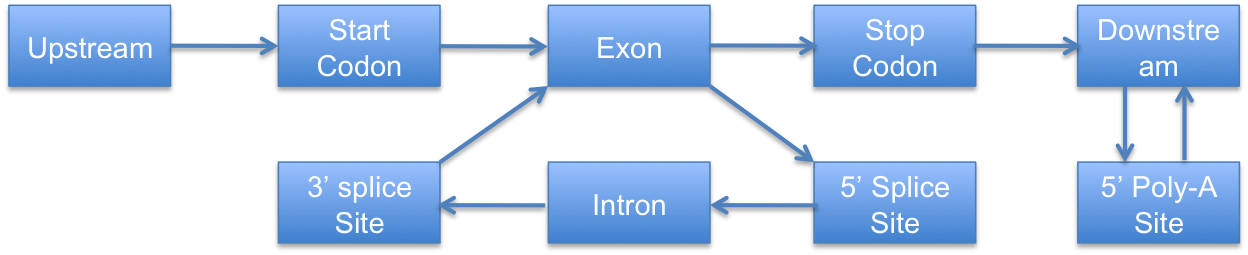
\includegraphics[width=1.0\textwidth]{../picturesforthepresentation/combinedHMM.png}
	\end{figure}
	
	\begin{itemize}
		\item $\#$States=$94$, $\#$Transitions=$218$
		\item 5' Splice sites are 9-stage models
		\item 3' Splice sites are 15-stage models
	\end{itemize}
	
	\pause\begin{center}
		\textbf{The different models work like autonomous HMMs}
	\end{center}
	
\end{frame}

\begin{frame}
\frametitle{Explanation of the multiple-stage models}
	\begin{figure}
		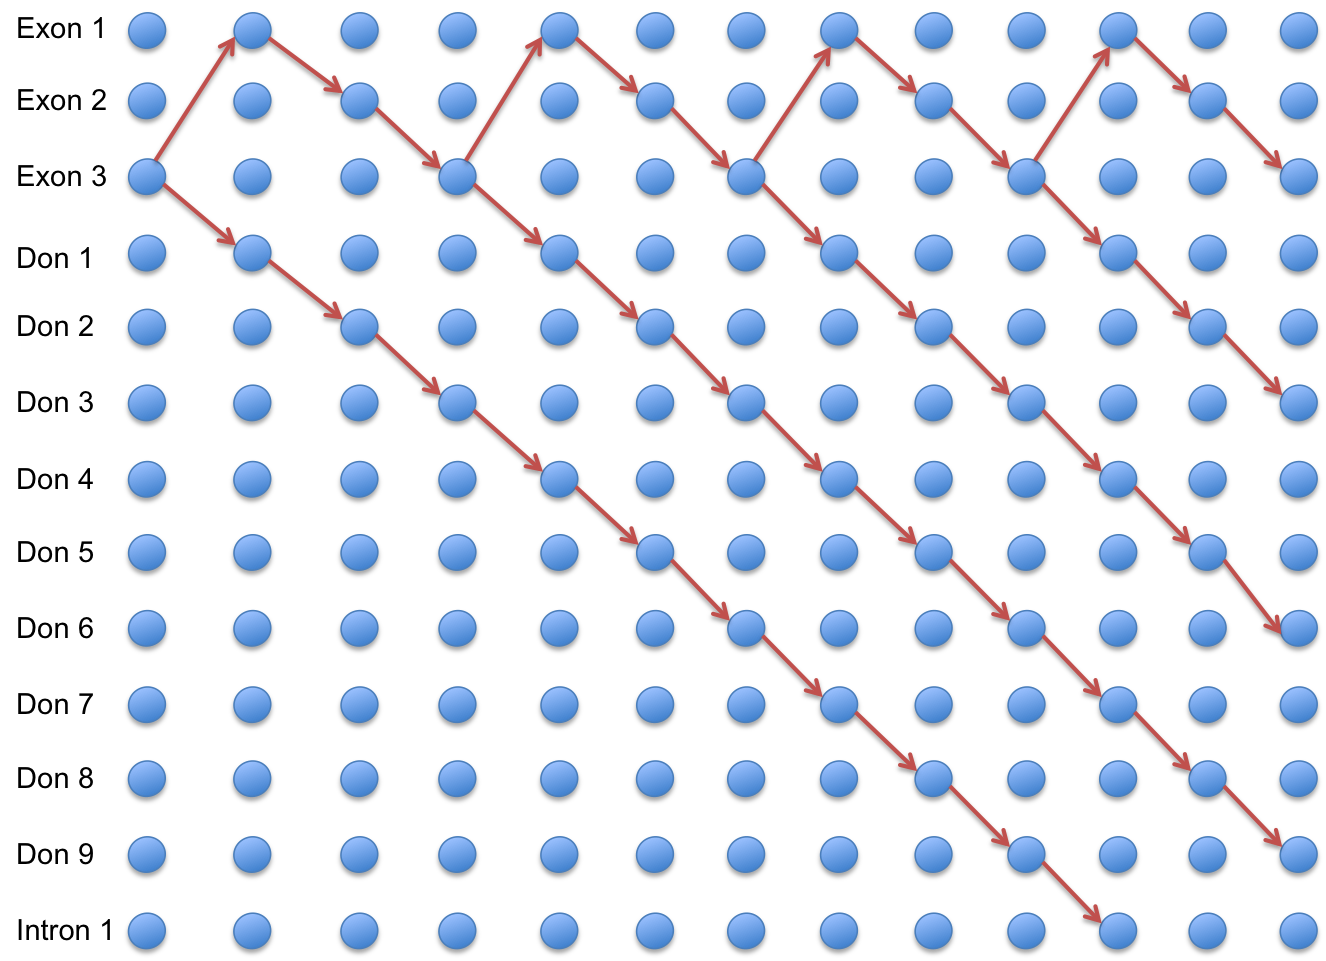
\includegraphics[width=0.9\textwidth]{../picturesforthepresentation/Stages_viterbi.png}
	\end{figure}
	
\end{frame}


\begin{frame}
\frametitle{Automaton Representation}
	\begin{figure}
		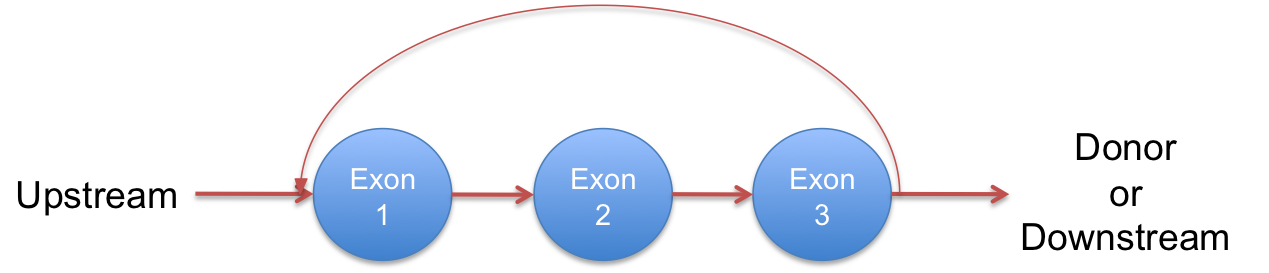
\includegraphics[width=1.0\textwidth]{../picturesforthepresentation/exon_auto.png}
	\end{figure}
	\begin{figure}
		\includegraphics[width=1.0\textwidth]{../picturesforthepresentation/donnor_auto.png}
	\end{figure}
	\pause\begin{center}
		\textbf{The donnor model is only a chain}
	\end{center}
\end{frame}


\begin{frame}
\frametitle{Additional structure information: The Poly-A site model}
	\begin{figure}
		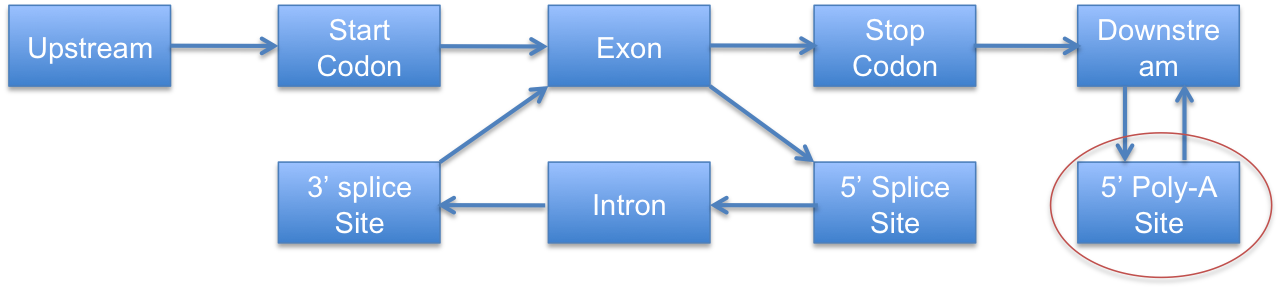
\includegraphics[width=1.0\textwidth]{../picturesforthepresentation/PolyA.png}
	\end{figure}
	
	\textbf{A concensus sequence : A A A T A A}
	
	\begin{itemize}
		\item A six-stage Markov chain
		\item One emission possibility of probability one for each stage 
		\item Needs almost no training 
	\end{itemize}
	
	\textbf{Start and Stop codon behave similarly}
\end{frame}

\begin{frame}
	\frametitle{Model limitations}
	\begin{columns}
		\begin{column}{6.5cm}
			Assumptions
			\begin{enumerate}
				\item Exon starts with a start codon
				\item Introns always flanked by exons
				\item Sequences contain exactly one gene
				\item Minimum length of a coding exon is 7
			\end{enumerate}
		\end{column}
		\begin{column}{4.5cm}
			
\includegraphics[width=4cm]{../picturesforthepresentation/restrictions.jpg}
		\end{column}
	\end{columns}
\end{frame}

\section{Implementation}

\begin{frame}
	\frametitle{General properties}
	\begin{columns}
		\begin{column}{6cm}
			\begin{itemize}
				\item General HMM framework
				\item Backward-, forward-, Viterbi and Baum-Welch Algorithm
				\item Support of silent states
				\item Persistency
			\end{itemize}
		\end{column}
		\begin{column}{5cm}
			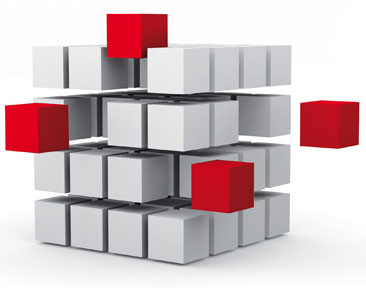
\includegraphics[width=4.5cm]{../picturesforthepresentation/features.jpg}
		\end{column}
	\end{columns}
\end{frame}

\begin{frame}
	\frametitle{Log-space transformation}
	\begin{itemize}
		\item Long sequences entail small probabilities $\Rightarrow$ Numerical instability and cancellation
		\item Solution: Logarithm transformation
	\end{itemize}
	\begin{block}{Products}
		\begin{displaymath}
			\log(a*b) = \log(a)+\log(b)
		\end{displaymath}
	\end{block}
	
	\begin{block}{Sums}
		\begin{displaymath}
			\log(a+b) = \log(a) + \log\left(1 + \exp\left(\log(a)-\log(b)\right)\right)
		\end{displaymath}
	\end{block}
\end{frame}

\begin{frame}
	\frametitle{Sum formula derivation}
	
	\begin{eqnarray*}
		\log(a+b) &=& \log\left(a(1+\frac{b}{a}) \right)\\
			&=& \log(a) + \log(1+\frac{b}{a})\\
			&=& \log(a) + \log(1+\exp\left( \log(b) - \log(a) \right))
	\end{eqnarray*}
	\begin{itemize}
		\item with $a>b$
	\end{itemize}
\end{frame}

\begin{frame}
	\frametitle{Model sparseness}
	\begin{columns}
		\begin{column}{6.5cm}
			\begin{itemize}
				\item Complexity of naive Baum-Welch $O(N\cdot K^2)$, $N$ length of sequence, $K$ number of states
				\item Too slow for given dataset
				\item Transition matrix sparse
				\item Average $\#$transitions$\approx 2$
				\item For our model: Linear time complexity in states $O(N\cdot K)$
			\end{itemize}
		\end{column}
		\begin{column}{4.5cm}
			\begin{figure}
				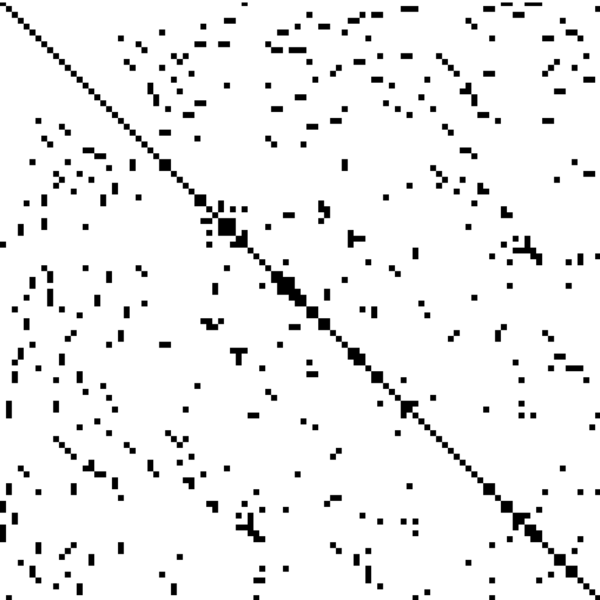
\includegraphics[width=4cm]{../picturesforthepresentation/sparse.png}
			\end{figure}
		\end{column}
	\end{columns}
\end{frame}

\section{Results}
\subsection{Database}
\begin{frame}
	\frametitle{Database}
	\begin{itemize}
		\item Created by Burset and Guigo (1996) "Evaluation of gene structure prediction programs."
		\item Selected sequences from GenBank
		\item Sequences fulfill assumptions
		\item 570 vertebrate sequences, 2649 exons and 2079 introns
		\item Total size of $2.9$MB
	\end{itemize}
\end{frame}

\subsection{Evaluation criteria}
\begin{frame}
\frametitle{Evaluation criteria}
	\begin{description}
		\item[Nucleotide sensitivity] Percentage of correctly labeled intron and exon bases
		\item[Nucleotide specificity] Percentage of correctly labeled exon bases
		\item[Exon sensitivity] Percentage of exons whose start and ending region has been correctly predicted
		\item[Exon specificity] Percentage of whole exons which are predicted exactly
	\end{description}
\end{frame}

\subsection{Overview of the results}

\begin{frame}
\frametitle{Non annotated learning}
\begin{columns}

		\column{0.50\textwidth}
		\begin{scriptsize}
		\begin{table}[h!]
		
		\begin{tabular}{|c|c|c|c|c|}
		
			\hline
				&Nucleotide sn	& Nucleotide sp\\	
			\hline
				Test set 1	& 0.693774	& 0.681791\\
			\hline
				Test set 2	& 0.663321	& 0.664126\\
			\hline
				Test set 3	& 0.664092	& 0.720411\\
			\hline
				Test set 4	& 0.637952	& 0.697138\\
			\hline
				Test set 5	& 0.674304	& 0.730396\\
			\hline
				Avg		& 0.6666886	& 0.6987724\\
			\hline	
			
					
		\end{tabular}
		\vspace{0.5 cm}
		
		\begin{tabular}{|c|c|c|c|c|}
		
			\hline
				& Exon sn	& Exon sp\\
			\hline
				Test set 1& 0.294624	& 0.243011\\
			\hline
				Test set 2	& 0.294231	& 0.259615	\\
			\hline
				Test set 3	& 0.315596	& 0.275229\\
			\hline
				Test set 4	& 0.402262	& 0.357027\\
			\hline
				Test set 5	& 0.314		& 0.272\\
			\hline
				Avg		& 0.3241426	& 0.2813764\\
			\hline	
			
					
		\end{tabular}
		
		%\caption{Exons}
		\end{table}
		

		\end{scriptsize}
		
		\column{0.50\textwidth}
		
		\begin{itemize}
			\item Test set size=$114$
			\item $3$ tries per test set
			\item Termination criterium: Threshold $\sigma=0.01$
			\item Convergence after 39 iterations on average
		\end{itemize}
		\vspace{0.5 cm}
		 
		 \centering\textbf{How to improve ? Partially supervised learning}
\end{columns}


\end{frame}

\begin{frame}
\frametitle{Annotated learning}
\begin{columns}

		\column{0.50\textwidth}
		\begin{scriptsize}
		\begin{table}[h!]
		
		\begin{tabular}{|c|c|c|c|c|}
		
			\hline
				&Nucleotide sn	& Nucleotide sp\\	
			\hline
				Test set 1	& 0.891234	& 0.743971\\
			\hline
				Test set 2	& 0.888242	& 0.723441\\
			\hline
				Test set 3	& 0.886976	& 0.791392\\
			\hline
				Test set 4	& 0.889267	& 0.745932\\
			\hline
				Test set 5	& 0.896504	& 0.81004\\
			\hline
				Avg		& 0.8904446	& 0.7629552\\
			\hline	
			
					
		\end{tabular}
	
		\vspace{0.5 cm}
		
		\begin{tabular}{|c|c|c|c|c|}
		
			\hline
				& Exon sn	& Exon sp\\
			\hline
				Test set 1 & 0.550538	& 0.539785\\
			\hline
				Test set 2	& 0.540385	& 0.530769	\\
			\hline
				Test set 3	& 0.588991	& 0.581651\\
			\hline
				Test set 4	& 0.621971	& 0.613893\\
			\hline
				Test set 5	& 0.586		& 0.586\\
			\hline
				Avg		& 0.577577	& 0.5704196\\
			\hline	
			
					
		\end{tabular}
		
		%\caption{Exons}
		\end{table}
		
		\end{scriptsize}
		
		\column{0.50\textwidth}
		%\begin{block}{With non-annotated leaning}<1>
		
		\begin{itemize}
			\item Test set size=$114$
			\item Termination criterium: Threshold $\sigma=0.01$
			\item Convergence after 18 iterations on average
			\item Results comparable with literature
		 \end{itemize}
		 
		 \vspace{0.5 cm}
		 
		 \centering\textbf{Much better accuracy}
\end{columns}
\end{frame}

\section*{}
\subsection{Conclusion}

\begin{frame}
\frametitle{Conclusion}
How to analyze the huge quantity of data provided by high-throughput sequencing ? 

\begin{itemize}
		\item Statistical models
		\item Artificial intelligence and self-trained models
		\item Injection of biological informations 
		 \end{itemize}
		 
		 \vspace{0.5 cm}
		 
		 \pause \begin{center}\textbf{Another way of injecting biological information : pair hidden Markov
model for comparative gene finding (Homology)}\end{center}
\end{frame}

\begin{frame}[allowframebreaks]
  \frametitle<presentation>{Bibliography}    
  \begin{thebibliography}{10}   
	\beamertemplatearticlebibitems
	\bibitem{}
	J.~Henderson, S.~Salzberg, K.~Fasman
	\newblock Finding Genes in DNA with a Hidden Markov Model, 1997
	
	\beamertemplatearticlebibitems
	\bibitem{}
	W.~Majoros, M.~Pertea, S.~Salzberg
	\newblock Efficient implementation of a generalized pair hidden Markov model for comparative gene finding, 2005

	\bibitem{}
	L.~Stein
	\newblock Genome Annotation: From sequence to biology, 2001
	
	\bibitem{}
	B.~Yoon
	\newblock Hidden Markov Models and their Applications in Biological Sequence Analysis, 2009

	\bibitem{}
	S.~Maji, D.~Garg  	
	\newblock Progress in Gene Prediction: Principles and Challenges, 2013
	
	\bibitem{}
	R.~Sleator 	
	\newblock An overview of the current status of eukaryote gene prediction strategies, 2010

	\bibitem{}
	A.~Lomsadze, V.~Ter-Hovhannisyan, Y.~Chernoff, M.~Borodovsky
	\newblock Gene identification in novel eukaryotic genomes by self-training algorithm, 2005

	\bibitem{}
	R.~Azad, M.~Borodovsky
	\newblock Probabilistic methods of identifying genes in prokaryotic genomes: Connections to the HMM theory, 2004

	\bibitem{}
	M.~Zhang
	\newblock Computational prediction of eucaryotic protein-coding genes, 2002

	\bibitem{}
	C.~Burge, S.~Karlin
	\newblock Prediction of complete gene structures in human genomic DNA, 1997  	
  \end{thebibliography}
\end{frame}


\end{document}
